% =====================================================================
%  SECTION 7 — Quadrature safety: predicting collocation overfitting
%  Draft 1. Every number is traceable to RESULTS.md and regenerable
%  from a seeded script in examples/.
% =====================================================================

\section{Quadrature safety: predicting collocation overfitting}
\label{sec:quadrature}

The certificates of Sections~\ref{sec:primaldual}--\ref{sec:exact} are
statements about integrals. Any practical scheme evaluates those integrals
approximately during training, and the resulting bound inherits the
quadrature error. This section characterises when that error is benign,
when it is fatal, and how to detect the difference \emph{without access to
a reference solution}.

\subsection{The phenomenon and what is already known}
\label{sec:quad:prior}

That a collocation-evaluated loss can be arbitrarily misleading is
established. Berrone, Canuto and Pintore~\cite{Berrone2022} construct a
nonzero network whose variational loss vanishes at every quadrature point
while its error remains of order one, and derive a sufficient condition
based on \emph{polynomial precision}: the quadrature rule must be exact for
polynomials of degree at least twice that of the test space. Within
homogenization specifically, Gaynutdinova et al.~\cite{Gaynutdinova2026}
report the effect empirically for both spectral and neural test functions:
enlarging the test basis lowers the training loss substantially while
\emph{degrading} the resulting estimates, an effect they attribute to
overfitting the imprecision of the numerical integration, and which is
worse for higher-frequency bases. They also observe the primal--dual gap
converging while further optimisation merely fits the test functions.

A separate and active literature addresses collocation placement directly,
through residual-adaptive refinement and related schemes. That work is
complementary to what follows rather than competing with it: adaptive
sampling is a \emph{training} strategy that redistributes points towards
large residuals, whereas the criterion below is a \emph{post-training} test
of whether a given rule was adequate for the field that was actually
learned. A practitioner may reasonably use both.

Neither the polynomial-precision criterion nor the empirical observation
answers the question a practitioner faces: \emph{given this trained
network, is my quadrature rule adequate?} Polynomial precision is not
directly applicable when the trial space is a neural network with no
polynomial degree, and an empirical observation identifies the failure only
after a reference solution has revealed it. Our contribution is therefore
not the discovery of the phenomenon but its \emph{prediction} and
\emph{prescription}: a computable criterion that flags the failure before
certification degrades, and that specifies how to choose the collocation
density.

\subsection{A computable criterion}
\label{sec:quad:criterion}

Let $u_\theta$ denote a trained periodic field and let $\hat u_\theta(\xi)$
be its discrete Fourier transform on a fine probe grid. Define the
\emph{spectral bandwidth} $B$ as the smallest radius containing a fraction
$q$ of the spectral energy excluding the mean,
%
\begin{equation}
  B \;=\; \min\Big\{ R : \textstyle\sum_{0<|\xi|\le R} |\hat u_\theta(\xi)|^2
  \;\ge\; q \sum_{\xi \neq 0} |\hat u_\theta(\xi)|^2 \Big\},
  \qquad q = 0.999 .
  \label{eq:bandwidth}
\end{equation}
%
A tensor-product midpoint rule with $n_q$ points per direction resolves
frequencies up to the Nyquist limit $n_q/2$. We define the \emph{headroom}
%
\begin{equation}
  h \;=\; \frac{n_q/2}{B},
  \label{eq:headroom}
\end{equation}
%
and, as an independent check requiring no spectral analysis, the
\emph{refinement ratio}
%
\begin{equation}
  \rho \;=\; \frac{\mathcal{E}_{4 n_q}(u_\theta)}{\mathcal{E}_{n_q}(u_\theta)},
  \label{eq:ratio}
\end{equation}
%
where $\mathcal{E}_{m}$ denotes the energy evaluated with $m$ points per
direction. Both quantities are computed from the trained network alone: no
exact solution, no reference solver, and no held-out labels are required.
This is the property that matters in practice, since the situation in which
the diagnostic is needed is precisely the situation in which no reference
exists.

\subsection{Empirical characterisation}
\label{sec:quad:empirical}

Table~\ref{tab:headroom} sweeps $n_q$ and the embedding richness for a
two-phase laminate of contrast~$6$, whose exact effective tensor has trace
$7.4167$. The behaviour is sharply thresholded at $h = 1$.

\begin{table}[t]
\centering
\caption{Headroom governs the reliability of a collocation-trained energy.
Laminate, contrast~6, width~48, depth~3, $400$ steps. ``Reported'' is the
energy at the training rule; ``refined'' at $4n_q$. Exact trace $7.4167$.}
\label{tab:headroom}
\resizebox{\textwidth}{!}{%
\begin{tabular}{rrrrrrrl}
\toprule
$n_q$ & harmonics & $B$ & $n_q/2$ & $h$ & reported & refined & $\rho$ \\
\midrule
 16 &  4 & 16.0 &  8.0 & 0.50 & 0.031 & 109.853 & 3498.46 \\
 32 &  4 &  9.0 & 16.0 & 1.78 & 7.271 &   7.921 &    1.09 \\
 64 &  4 &  7.0 & 32.0 & 4.57 & 7.394 &   7.612 &    1.03 \\
128 &  4 &  6.0 & 64.0 &10.67 & 7.434 &   7.446 &    1.00 \\
\midrule
 32 &  2 & 36.0 & 16.0 & 0.44 & 4.767 & 102.982 &   21.60 \\
 32 &  8 & 30.0 & 16.0 & 0.53 & 4.758 &  46.811 &    9.84 \\
 32 & 12 & 34.0 & 16.0 & 0.47 & 0.015 &  16.524 & 1093.23 \\
\bottomrule
\end{tabular}}

\end{table}

Figure~\ref{fig:headroom} collects these measurements together with
those of Section~\ref{sec:quad:universal}. Two regimes are evident. For $h < 1$ the reported energy is not merely
inaccurate but meaningless: refinement raises it by factors between $10$
and $3.5\times 10^{3}$, and in the worst case a reported value of $0.015$
corresponds to a true value near $16.5$. For $h > 1$ the ratio $\rho$
returns to unity, and a strictly valid midpoint bound required $h$ of order
ten in this configuration.

We note in passing that $B$ is \emph{not} monotone in the richness of the
Fourier embedding: it is minimised at four harmonics and substantially
larger at both two and twelve. An under-parameterised embedding cannot
represent the target smoothly, so optimisation inflates the weights and the
$\tanh$ nonlinearity manufactures high harmonics; an over-parameterised one
is simply free to oscillate. Both extremes therefore degrade headroom, and
tuning the embedding without simultaneously revisiting $n_q$ is unsafe.


\begin{figure}[t]
\centering
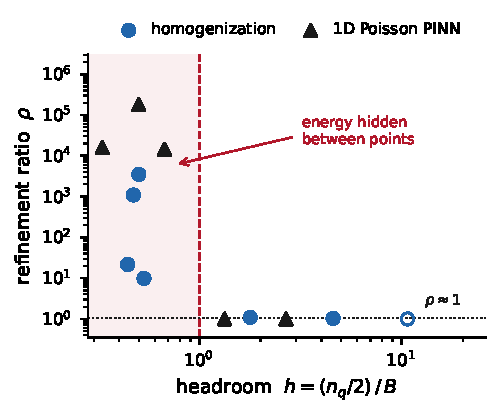
\includegraphics[width=\linewidth]{figures/fig_headroom.pdf}
\caption{Headroom predicts collocation overfitting. Filled markers denote configurations whose reported energy failed to bound the exact value. The threshold at $h=1$ reproduces on a 1D Poisson PINN unrelated to homogenization.}
\label{fig:headroom}
\end{figure}

\subsection{Consequence for certification}
\label{sec:quad:false}

Low headroom does not merely widen a certificate: it can invalidate one.
Training a primal field against a fixed $32$-point rule on the laminate
above produced a reported upper bound of $2.5207$ against an exact value of
$2.6667$: a bound below the quantity it purports to bound. In an
adversarially trained case the reported upper bound was $0.0014$ against an
exact value of $3.0769$, with refinement revealing a true energy near
$58.9$. Both failures are silent: the training loss is small and
monotone, and the fields are visually unremarkable.

Exact-integration certification (Section~\ref{sec:exact}) removes the
failure mode entirely rather than mitigating it. Interpolation onto a
conforming finite-element space followed by element-exact Gauss quadrature
cannot hide energy between sample points, because the integral has no
sample points between which to hide it. Every certificate reported in this
work is obtained in this way; midpoint values are used only as training
diagnostics. On the laminate case above, the exactly integrated bound is
$3.0429$, correctly above the exact value that the collocation-trained
estimate violated.

\subsection{The failure is not specific to homogenization}
\label{sec:quad:universal}

To establish that the criterion characterises collocation training rather
than this particular problem, we repeat the measurement on a textbook
physics-informed network: $-u'' = f$ on $(0,1)$ with homogeneous Dirichlet
data imposed exactly by the ansatz $u_\theta = x(1-x)N_\theta(x)$, exact
solution $u^\star = \sin(\pi x)$, a plain $\tanh$ multilayer perceptron,
and a residual-only loss on $N$ fixed collocation points.

\begin{table}[t]
\centering
\caption{Collocation overfitting in a vanilla PINN on 1D Poisson. The
reported residual is evaluated at the training points; the honest residual
on a $20\times$ finer grid. Bandwidth $6.0$ throughout.}
\label{tab:pinn}
\resizebox{\textwidth}{!}{%
\begin{tabular}{rrrrrr}
\toprule
$N$ & residual (train) & residual (fine) & $\rho$ & $h$ & $L^2$ error \\
\midrule
 4 & $2.84\times10^{-5}$ & $4.51\times10^{-1}$ & $1.59\times10^{4}$ & 0.33 & 1.06\% \\
 6 & $1.55\times10^{-6}$ & $2.83\times10^{-1}$ & $1.83\times10^{5}$ & 0.50 & 0.17\% \\
 8 & $1.14\times10^{-6}$ & $1.66\times10^{-2}$ & $1.46\times10^{4}$ & 0.67 & 0.00\% \\
16 & $2.10\times10^{-1}$ & $2.10\times10^{-1}$ & $1.00$            & 1.33 & 0.77\% \\
32 & $2.25\times10^{-3}$ & $2.27\times10^{-3}$ & $1.00$            & 2.67 & 0.00\% \\
\bottomrule
\end{tabular}}

\end{table}

A reported residual of $1.55\times10^{-6}$, which in a loss curve is
indistinguishable from convergence to machine precision---corresponds to a
true residual of $0.283$. The threshold reproduces exactly: every
configuration with $h<1$ overfits, and every configuration with $h>1$ has
$\rho = 1.000$. We stress the honest reading of this table: because the
problem is easy and the boundary conditions are imposed exactly, the
\emph{solution} remains accurate even where the reported residual is
meaningless. The failure is thus epistemic rather than always catastrophic: the training residual cannot be used as evidence of
convergence---which is precisely the situation of a practitioner with no
analytic solution to check against.

\subsection{A per-run, label-free quality gate}
\label{sec:quad:gate}

Headroom is a property of the \emph{trained field}, not of the
configuration. At fixed architecture, fixed $n_q = 64$ and fixed data,
five independently seeded trainings of the laminate case produced
bandwidths of $7.0$, $6.0$, $7.0$, $41.0$ and $6.4$: four runs at
$h \approx 4.9$ with certified gaps between $0.4\%$ and $1.7\%$, and one
run at $h = 0.78$ with a certified gap of $97.8\%$ and $\rho = 7.076$. Both
diagnostics fired on exactly the failing run and on none of the others,
without reference to the exact tensor.

We therefore accept a trained field when
%
\begin{equation}
  h \ \ge\ 2 \qquad\text{and}\qquad \rho \ \le\ 1.05 ,
  \label{eq:gate}
\end{equation}
%
and otherwise reject it, retraining or increasing $n_q$. We emphasise that
a rejected run is not an invalid one: certified by exact integration it
still provably contains the truth, and validity held in all five seeds
above including the rejected one. The gate separates trustworthy
\emph{tightness} from guaranteed \emph{validity}, a distinction that only
a certified method can express, and which an uncertified surrogate cannot
even formulate.

A further consequence is a stopping criterion. Overfitting accumulates: the
collapse above appeared between $250$ and $400$ optimisation steps, all
five seeds being clean at the earlier budget. Training longer is therefore
not monotonically better, and~\eqref{eq:gate} supplies a signal that the loss curve cannot: stop when headroom degrades, not when the loss
plateaus.

\subsection{Prescriptive use}
\label{sec:quad:prescription}

The criterion also determines how to configure a run. Consider the
bicontinuous morphology of Section~\ref{sec:limits}, generated as the level
set of a filtered Gaussian field with dominant wavenumber six. With four
embedding harmonics the trial space cannot represent the microstructure's
own length scale, and the certified gap is $50.4\%$. Enriching the
embedding tightens the bound monotonically but consumes headroom, until the
gate rejects the result:

\begin{table}[t]
\centering
\caption{Trial-space richness and quadrature resolution are coupled
requirements. Bicontinuous morphology, contrast $10$.}
\label{tab:prescription}
\resizebox{\textwidth}{!}{%
\begin{tabular}{rrrrrl}
\toprule
harmonics & $n_q$ & certified gap & tightening & $h$ & gate \\
\midrule
 4 &  64 & 50.4\% & 2.0$\times$ & 2.86 & accept \\
12 &  64 & 29.9\% & 3.3$\times$ & 1.48 & \textbf{reject} \\
12 & 128 & 33.2\% & 3.0$\times$ & 3.16 & accept \\
\bottomrule
\end{tabular}}

\end{table}

The middle row is instructive. It reports the tightest gap of the three and
is nonetheless untrustworthy; the honest configuration reports $33.2\%$.
The $3.3$ percentage points separating them are quadrature illusion, and
the gate identifies this with no reference solution. Without the criterion,
$29.9\%$ is the number that would have been published.

This yields a concrete recipe. Estimate the dominant wavenumber $k$ of the
microstructure; choose the embedding richness so that the trial space
resolves it, $n_{\mathrm{harm}} \gtrsim 2k$; measure the bandwidth $B$ of
the trained field and set $n_q \ge 4B$; then verify~\eqref{eq:gate} and
iterate if it fails. Tuning either quantity in isolation is unsafe.

\subsection{Scope}
\label{sec:quad:scope}

The thresholds in~\eqref{eq:gate} are empirical, calibrated on the problems
reported here; we do not claim them as universal constants, and a
practitioner adopting the criterion should recalibrate on a case with a
known solution. The bandwidth~\eqref{eq:bandwidth} is defined for periodic
fields and requires modification for non-periodic problems, where spectral
leakage contaminates the estimate. The refinement ratio~\eqref{eq:ratio} is
free of both limitations and costs one additional energy evaluation; where
only one diagnostic can be afforded, it is the one to compute.
